\documentclass[openany]{book}
\usepackage[utf8]{inputenc}
\usepackage{verbatim}
\usepackage[hypertexnames=false]{hyperref}
\usepackage{amstext} 
\usepackage{array}   
\newcolumntype{C}{>{$}c<{$}} 


%%%%%%%%%%%%%%%%%%%%%%%

%%%%%%%%%%%%%%%%%%%%%%%
% HOLA PACO
% ESTE ES EL ARCHIVO DE LAS DEFINICIONES ESTRUCTURALES
% VERSION 1.1 NOMÁS
%
% AUTOR ORIGINAL:
% EDUARDO (CHITO) BELMONTE GUILLAMÓN
%
% ESTE ARCHIVO ES COMUNISTA, PUEDES COMPARTIRLO SI QUIERES
%%%%%%%%%%%%%%%%%%%%%%%

%----------------------------------
%     PAQUETICOS QUE SE USAN
%----------------------------------

%--------------------------
%    PARA USAR INKSCAPE
%---------------------------
\usepackage{import}
\usepackage{hyperref}
\usepackage{xifthen}
\usepackage{pdfpages}
\usepackage{transparent}

\newcommand{\incfig}[1]{%
    \def\svgwidth{\columnwidth}
    \import{./figures/}{#1.pdf_tex}
}

\newcommand{\custincfig}[2]{%
    \def\svgwidth{#1}
    \import{./figures/}{#2.pdf_tex}
}
\newcommand{\textnexttofig}[3]{
  \begin{minipage}[l]{0.45\textwidth}
    \custincfig{#1}{#2}
  \end{minipage}
  \begin{minipage}[l]{0.45\textwidth}
    #3
  \end{minipage}
}

%%%%%%%%% FIN DEL INKSCAPE

\usepackage{parskip} % Pa parrafos wapos
\setlength{\parindent}{0.5cm} % Pa la sangría
\usepackage{graphicx} % Pa meter las imágenes
\graphicspath{{Images/}} % La ruta a las imágenes

\usepackage{tikz} % Pa dibujar cosichuelas guapas

\usepackage[spanish]{babel} % PA QUE ESTÉ EN ESPAÑOL NOMÁS

\usepackage{enumitem} % Para personalizar las LISTAS YEAH

\setlist{nolistsep} % Pa que las listas estén junticas

\usepackage{booktabs} % Esta sirve para hacer tablas fancy con multicolumns y tal pero no tengo ni puta idea de usarla

\usepackage{xcolor} % PA DEFINIR LOS COLORINES
\definecolor{turquoise}{RGB}{21,103,112} % Es un turquesica así formal
\definecolor{violet}{RGB}{ 110, 6, 187 } % Color maricón

%-------------------------------------------------
%     MÁRGENES
%-------------------------------------------------

\usepackage{geometry}
\geometry{
    top=3cm,
    bottom=3cm,
    left=3cm,
    right=3cm,
    headheight=14pt,
	footskip=1.4cm,
	headsep=10pt,
}

\usepackage{avant} % Esto es una fuente para encabezados

%\usepackage{mathptmx} % Usar simbolitos matemáticos chulos

\usepackage{microtype} % Para fuentes de maricones

\usepackage[utf8]{inputenc} % Pa los acentos

\usepackage[T1]{fontenc}

%-------------------------------------------------
% Bibliografía e índice
%-------------------------------------------------

\usepackage{makeidx} % Pa hacer un índice
\makeindex

\usepackage{titletoc}   % Para manipular la tabla de contenidos

\contentsmargin{0cm}    % Para eliminar el margen por defecto

\usepackage{titlesec} % Pa cambiar los titulos skere

\titleformat
{\chapter} % command
[display] % shape
{\centering\bfseries\Huge\normalfont} % format
{\color{turquoise}  {\normalsize\MakeUppercase{Capítulo} \thechapter }} % label
{-0.5cm} % sep
{
    \color{turquoise}
    \rule{\textwidth}{3pt}
    \vspace{1ex}
    \centering
    \setcounter{ex}{0}
    \setcounter{dummy}{0}
} % before-code
[
\vspace{-0.5cm}%
\rule{\textwidth}{3pt}
] % after-code


\titleformat{\part}
[display]
{\centering\bfseries\Huge\normalfont}
{\color{turquoise} {\normalsize \MakeUppercase{Asignatura}}}
{0pt}
{\color{turquoise}
\vspace{-0.6cm}
\rule{\textwidth}{3pt}
\vspace{1ex}
\setcounter{chapter}{0}
\setcounter{section}{0}
\setcounter{dummy}{0}
\centering
}


\titleformat{\section}
{\normalfont\Large\bfseries}{\color{turquoise}\thesection\ - }{0.5em}{}

\usepackage{fancyhdr}   % Necesario para el encabezado y el pie de página

\pagestyle{fancy}   %Para modificar los encabezados
\fancyhf{}          %Para eliminar los encabezados y pies de página por defecto.
\fancyhead[LE,RO]{\sffamily\normalsize\thepage}
\fancyfoot[C]{Ampliación de Probabilidad}
%HACER

\usepackage{amsmath,amsfonts,amssymb,amsthm,cancel} % PARA LAS MATES

%   LINEA 199, HACER CAPULLADAS

\newtheoremstyle{turquoisebox}
{0pt} %Espacio encima
{0pt} %Espacio abajo
{\normalfont} % Fuente del cuerpo
{} % Cantidad de identado
{\small\ssfamily\color{turquoise}} % Fuente en la que pone "TEOREMA"
{:} % Puntuación tras el teorema
{0.25em} %Espacio tras el teorema
{\thmname{#1}\thmnumber{#2}} %No sé si esto funciona


\newcounter{dummy}
\newcounter{ex}
\newtheorem{teoremote}[dummy]{\color{turquoise}Teorema}
\newtheorem{propositiont}{\color{turquoise}Proposición}[section]
\newtheorem{lemmat}{\color{turquoise}Lema}[section]
\newtheorem{definitionT}{\color{turquoise}Definición}[section]
\newtheorem{exerciseT}[ex]{Ejercicio}
\newtheorem{examplote}[ex]{\color{turquoise}Ejemplo}
\newtheorem{methodT}[dummy]{\color{turquoise}Método}


\RequirePackage[framemethod=default]{mdframed} % Required for creating the theorem, definition, exercise and corollary boxes

%Caja de teoremas

\newmdenv[skipabove=7pt,
skipbelow=7pt,
backgroundcolor=black!5,
linecolor=turquoise,
innerleftmargin=5pt,
innerrightmargin=5pt,
innertopmargin=5pt,
leftmargin=0cm,
rightmargin=0cm,
linewidth=3pt,
innerbottommargin=5pt]{tBox}

\newmdenv[skipabove=7pt,
skipbelow=7pt,
backgroundcolor=black!5,
linecolor=turquoise,
innerleftmargin=5pt,
innerrightmargin=5pt,
innertopmargin=5pt,
leftmargin=0cm,
rightmargin=0cm,
linewidth=1pt,
innerbottommargin=5pt]{pBox}

\newmdenv[skipabove=7pt,
skipbelow=7pt,
backgroundcolor=violet!7,
linecolor=turquoise,
innerleftmargin=5pt,
innerrightmargin=5pt,
innertopmargin=5pt,
leftmargin=0cm,
rightmargin=0cm,
rightline=false,
topline=false,
bottomline=false,
linewidth=4pt,
innerbottommargin=5pt]{mBox}

\newmdenv[skipabove=7pt,
skipbelow=7pt,
rightline=false,
leftline=true,
topline=false,
bottomline=false,
linecolor=turquoise,
innerleftmargin=5pt,
innerrightmargin=5pt,
innertopmargin=0pt,
leftmargin=0cm,
rightmargin=0cm,
linewidth=4pt,
innerbottommargin=0pt]{dBox}

\newmdenv[skipabove=7pt,
skipbelow=7pt,
rightline=false,
leftline=true,
topline=false,
bottomline=false,
backgroundcolor=black!3,
linecolor=turquoise!50,
innerleftmargin=5pt,
innerrightmargin=5pt,
innertopmargin=0pt,
innerbottommargin=5pt,
leftmargin=0cm,
rightmargin=0cm,
linewidth=4pt]{eBox}

\newmdenv[skipabove=7pt,
skipbelow=7pt,
leftline=true,
topline=false,
rightline=false,
bottomline=false,
backgroundcolor=cyan!5,
linecolor=turquoise,
innerleftmargin=5pt,
innerrightmargin=5pt,
innertopmargin=0pt,
innerbottommargin=5pt,
leftmargin=0cm,
rightmargin=0cm,
linewidth=4pt]{exBox}

\newenvironment{theorem}{\begin{tBox}\begin{teoremote}}{\end{teoremote}\end{tBox}}
\newenvironment{proposition}{\begin{pBox}\begin{propositiont}}{\end{propositiont}\end{pBox}}
\newenvironment{lemma}{\begin{pBox}\begin{lemmat}}{\end{lemmat}\end{pBox}}
\newenvironment{method}{\begin{mBox}\begin{methodT}}{\end{methodT}\end{mBox}}
\newenvironment{definition}{\begin{dBox}\begin{definitionT}}{\end{definitionT}\end{dBox}}
\newenvironment{exercise}{\begin{eBox}\begin{exerciseT}}{\hfill{\color{black}}\end{exerciseT}\end{eBox}}
\newenvironment{example}{\begin{exBox}\begin{examplote}}{\end{examplote}\end{exBox}}
\newenvironment{demonstration}{\begin{flushright}
      \color{turquoise} \textbf{Demostración}
\end{flushright}
}{\begin{flushright}
  $\square$
\end{flushright}}

\usepackage{geometry}
\geometry{
    top=3cm,
    bottom=3cm,
    left=3cm,
    right=3cm,
    headheight=14pt, 
    footskip=1.4cm,
    headsep=10pt,
}
\usepackage{graphicx}
\title{Ejercicios de Ampliación de Probabilidad}
\author{Paco Mora Caselles}
\date{\today}

\begin{document}

\maketitle

\chapter{Relación 1}
\begin{exercise}
    $$  C = \{(x,y) \in \mathbb{R} ^2 \ :\ 0<x<1,\ 0<y<1,\ y < (1-x)^2\} $$

    \begin{center}
        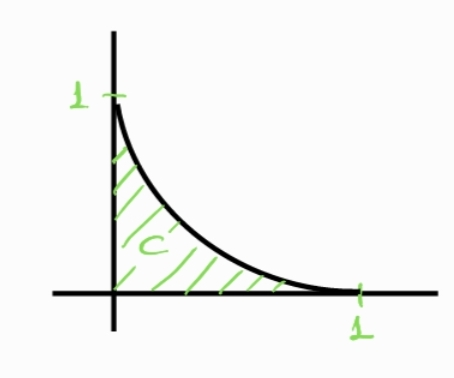
\includegraphics[scale=0.5]{1-1.jpg}
    \end{center}

    Dejamos por ahora $ f $ en función de $ k $, más tarde calculamos su valor:

    $$ f(x,y) = \left\{
    \begin{array}{lr}
        k & (x,y) \in C\\
        0 & (x,y) \not \in C   
    \end{array}
    \right. $$

    Para $ x \in (0,1) $:
    $$ f_{1}(x) = \int\limits_{}^{}f(x,y) dy = \int\limits_{0}^{(1-x)^2}k dy = k(1-x)^2 $$

    Entonces tenemos:

    $$ f_{1}(x) = \left\{
    \begin{array}{lr}
        k(1-x)^2 & x \in (0,1)\\
        0 & x \not \in (0,1)
    \end{array}
    \right. $$

    Pasamos ahora a $ f_{2}(y) $, cuando $ y \in (0,1) $:
    $$ f_{2}(y) = \int\limits_{}^{}f(x,y)dx = \int\limits_{0}^{1-y^{1/2}} = k (1-y)^{1/2} $$

    $$ f_{2}(y) = \left\{
    \begin{array}{lr}
        k(1-\sqrt{y}) & y \in (0,1) \\
        0 & y \not \in (0,1)
    \end{array}
    \right. $$

    Calculamos ahora $ E(X^{n}(1-X)^{m}) $ usamos $ f_{1}(x) $:
    $$ E(X^{n}(1-X)^{m}) = \int\limits_{}^{}x^{n}(1-x)^{m}f_{1}(x)dx = \int\limits_{0}^{1} x^{n}(1-x)^{m} k (1-x)^2 dx = k \int\limits_{0}^{1}x^{n}(1-x)^{m+2} =$$
    $$ =  kB(n+1,m+3) = k \dfrac{\Gamma(n+1)\Gamma(m+3)}{\Gamma(n+m+4)} = k \dfrac{n!(m+2)!}{(n+m+3)!} $$
    
    Los momentos de orden $ n $ respecto del origen, la esperanza y la varianza de $ X $ las podemos calcular con esta expresión. Para los primeros casos tomamos $ m=0 $ y para la varianza podemos usar que $ Var(X) = E(X^2)-E(X)^2 $

    $$ k = 3 \hspace{10mm} E(X) = \dfrac{1}{4}\hspace{10mm} E(X^2) = \dfrac{1}{10} \hspace{10mm} Var(X) = \dfrac{3}{80} $$
    
    Calculamos $ f_{2|1}(y|x) $, si $ x \in (0,1) $:
    $$ f_{2|1}(y|x) = \dfrac{f(x,y)}{f_{1}(x)} = \left\{
    \begin{array}{lr}
        \dfrac{3}{3(1-x)^2} = \dfrac{1}{(1-x)^2} & y \in (0,(1-x)^2)\\
        0 & y \not \in (0,(1-x)^2)
    \end{array}
    \right. $$

    Podemos calcular ahora $ f_{2|1}(y|x=1/2) $:
    $$ f_{2|1}(y|1/2) = \left\{
    \begin{array}{lr}
        4 & y \in (0,\dfrac{1}{4}) \\\\
        0 & y \not \in (0,\dfrac{1}{4})
    \end{array}
    \right. $$

    Para calcular $ F\left(\dfrac{1}{4},\dfrac{9}{16}\right) $ nos apoyamos en la figura para saber que basta con calcular el área del rectángulo y multiplicar por $ k $:
    
    \begin{center}
        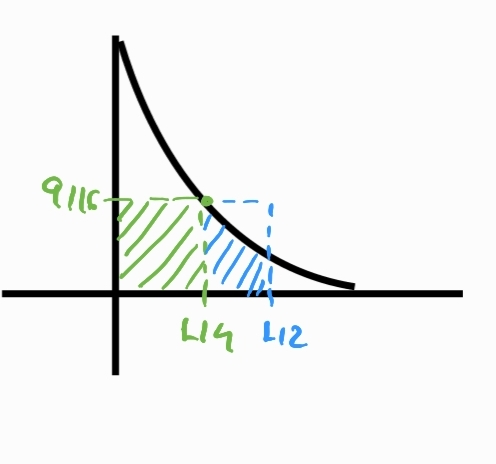
\includegraphics[scale=0.4]{1-1-2.jpg}
    \end{center}
    

    $$ F\left(\dfrac{1}{4},\dfrac{9}{16}\right) = 3 \dfrac{1}{4}\cdot \dfrac{9}{16} = \dfrac{3^3}{2^{6}}$$

    Para $ F\left(\dfrac{1}{2},\dfrac{9}{16}\right) = F\left(\dfrac{1}{4},\dfrac{9}{16}\right)+3\cdot Area\ T $, siendo $ T $ la intersección con $ C $. Sabemos entonces que:
    $$ \int\limits_{1/4}^{1/2}(1-x)^2dx = \int\limits_{1/4}^{1/2}(x^2-2x+1)dx = \dfrac{x^3}{3}-x^2+x \Biggr|_{1/4}^{1/2} = \dfrac{19}{2^{6}3} $$
    $$ F\left(\dfrac{1}{2},\dfrac{9}{16}\right) = \dfrac{3^3}{2^{6}} + 3 \dfrac{19}{2 ^{6}3} = \dfrac{23}{32} $$

    Tenemos que calcular ahora la recta de regresión de $ Y $ respecto de $ X $:
    $$ y - \mu_{y} = \dfrac{\sigma _{xy}}{\sigma_{x}^2}(x-\mu_{x}) $$
    $$ \mu_{y} = E(Y) = \int\limits_{0}^{1} y 3(1-y^{1/2})dy = 3 \int\limits_{0}^{1}(y-y^{3/2}) = \dfrac{3}{10} $$
    $$ E(XY) = \int\limits_{0}^{1} \int\limits_{0}^{(1-x)^2} 3xy dy dx = 3 \int\limits_{0}^{1} x \left[\dfrac{y^2}{2}\right]_{0} ^{(1-x)^2} d = \dfrac{3}{2} \int\limits_{0}^{1}x(1-x)^{4}dx = $$
    $$ = B(2,5) = \dfrac{3}{2} \dfrac{\Gamma(2)\Gamma(5)}{\Gamma(7)}= \dfrac{3}{2} \dfrac{1!4!}{6!} = \dfrac{1}{20} $$
    Recordemos que $ \mu_{X} = E(X) = \dfrac{1}{4} $, entonces:
    $$ \sigma_{XY}Cov(X,Y) = \dfrac{1}{2^2\cdot 5} -\dfrac{1}{2^2}\cdot \dfrac{3}{2\cdot 5} = \dfrac{2-3}{2^3\cdot 5} = -\dfrac{1}{2^3\cdot 5}$$

    Podemos expresar ya la recta de regresión (recordando que $ \sigma_{X}  = \dfrac{3}{80}$):
    $$ y-\dfrac{3}{10} = \dfrac{-1/(5\cdot 2^3)}{3/(2^{4}\cdot 5)}(x-\dfrac{1}{4}) $$
    $$ y = -\dfrac{2}{3}x+\dfrac{7}{15} $$

    Calculamos ahora $ E(Y|X=x) = m_{2|1}(x) $:
    $$ E(Y|X=x) = \int\limits_{}^{}y f_{2|1}(y|x)dy = \int\limits_{0}^{(1-x)^2}y \dfrac{1}{(1-x)^2}dy = $$
    $$ =\dfrac{1}{(1-x)^2} \dfrac{y^2}{2} \Biggr|_{0}^{(1-x)^2} = \dfrac{1}{(1-x)^2} \dfrac{(1-x)^{4}}{2} = \dfrac{(1-x)^2}{2} $$


\end{exercise}


\begin{exercise}
    $$ E(X) = 2,\ Var(X) = 3\ X\ \text{simétrica} $$
    
    $$ \alpha_{3} = E(X^3) = E((X-2+2)^3) = E((X-2)^3+3(X-2)^22+3(X-2)2^2+2^3) = $$
    $$= E((X-2)^3)+6E((X-2)^2) +12 E(X-2)+E(2^3) = 0 + 6 Var(X)+0+2^3 = 6\cdot 3+8 = 26$$
\end{exercise}


\begin{exercise}
    $  $
    El número de de posibilidades totales es claramente $ \binom{N}{n} $, la distribución de probabilidad es entonces:

    $$ P(X_1=r_1,X_2=r_2,X_3=r_3) = \dfrac{\binom{n_1}{r_1}\binom{n_2}{r_2}\binom{n_3}{r_3}}{\binom{N}{n}} $$
    Claramente necesitamos $ n\leq N,\ r_1+r_2+r_3=n $

    Calculamos ahora $ \alpha_{(3)} $:
    $$ E(X_1 ^{(3)}) = E(X_1(X_1-1)(X_1-2)) = \sum\limits_{r_1+r_2+r_3=n}^{}r_1(r_1-1)(r_1-2)\dfrac{\binom{n_1}{r_1}\binom{n_2}{r_2}\binom{n_3}{r_3}}{\binom{N}{n}} $$

    Nos fijamos que:

    $$r_1(r_1-1)(r_1-2)  \binom{N_1}{r_1} = r_1(r_1-1)(r_1-2) \dfrac{N_1 ^{(r_1)}}{r_1(r_1-1)(r_1-2)\cdots 2\cdot 1} = $$
    $$ =\dfrac{N_1 ^{(r_1)}}{(r_1-3)!} = N_1(N_1-1)(N_1-2) \dfrac{(N_1-3) ^{(r_1-3)}}{(r_1-3)!}  = N_1(N_1-1)(N_1-2)\binom{N_1-3}{r_1-3}$$

    Entonces volviendo a la igualdad anterior:
    $$ P(X_1=r_1) = \sum\limits_{r_1+r_2+r_3=n}^{}N_1(N_1-1)(N_1-2) \dfrac{\binom{N_1-3}{r_1-3}\binom{N_2}{r_2}\binom{N_3}{r_3}}{\binom{N}{n}} =  $$
    $$ N_1(N_1-1)(N_1-2)\sum\limits_{r_1+r_2+r_3=n}^{} \dfrac{\binom{N_1-3}{r_1-3}\binom{N_2}{r_2}\binom{N_3}{r_3}}{\binom{N}{n}} = N_1(N_1-1)(N_1-2) \dfrac{\binom{N-3}{n-3}}{\binom{N}{n}} =$$
    $$ = N_1(N_1-1)(N_2-2) \dfrac{(N-3) ^{(n-3)}n!}{(n-3)!N ^{(n)}} = \dfrac{N_1 ^{(3)}n ^{(3)}}{N ^{(3)}} $$
\end{exercise}


\begin{exercise}
    $  $

    \begin{flushright}
        \textbf{Aparado b)}
    \end{flushright}

    Para calcular las $ vvaa $ marginales solo tenemos que sumar los elementos de la misma fila o columna. Por ejemplo:

    $$ P(X=0) = \dfrac{1}{3}+\dfrac{1}{6}+\dfrac{1}{9} = \dfrac{11}{18} $$

    Obtenemos así:
    $$ P(X=0) = \dfrac{11}{18} \hspace{5mm} P(X=1) = \dfrac{5}{18} \hspace{5mm} P(X=2) = \dfrac{2}{18}$$
    $$ P(Y=0) = \dfrac{11}{18} \hspace{5mm} P(Y=1) = \dfrac{5}{18} \hspace{5mm} P(Y=2) = \dfrac{2}{18} $$

    También podemos obtener $ E(X) = E(Y) = \dfrac{1}{2} $, $ Var(X),Var(Y) = \dfrac{17}{36} $ y $ Cov(X,Y) = -\dfrac{5}{36} $.

    Entonces la recta de regresión de $ X $ sobre $ Y $ es:
    $$ Y-\mu_{Y} = \dfrac{\sigma_{XY}}{\sigma_{X}^2}(x-\mu_{X}) $$
    $$ y-\dfrac{1}{2} = \dfrac{-\dfrac{5}{36}}{\dfrac{17}{36}} \left(x-\dfrac{1}{2}\right) $$
    $$ y = -\dfrac{5}{17}x+\dfrac{11}{17} $$
    
    Como las esperanzas y las varianzas son iguales, obtenemos que el cálculo de la recta de regresión de $ Y $ sobre $ X $ es igual:
    $$ x = -\dfrac{5}{17}y+\dfrac{11}{17} $$

    Calcularemos ahora $ Var(Y-X^*) $:
    $$ Var(Y-X^* ) = \sigma_{Y}^2 (1-\rho ^2) = \dfrac{17}{36} \left( 1-\dfrac{25/36^2}{17^2/36} \right) = \dfrac{17}{36} \left( \dfrac{17^2-25}{17^2} = \dfrac{11}{3\cdot 17} \right) $$

    Para la varianza residual de $ X $ sobre $ Y $, vemos que es igual porque coinciden sus esperanzas y sus varianzas.


\end{exercise}


\chapter{Relación 2}

\begin{exercise}
    $  $
    Vemos en primer lugar cómo es el recinto del ejercicio:
    \begin{center}
        \includegraphics*[scale=0.5]{2-1-1.jpg}
        
    \end{center}
    
    $$ \alpha_{n.m} = E(X^{n}Y^{m}) = \int\limits_{}^{}x^{n}y^{m} \cdot  \dfrac{1}{y} = \int\limits_{0}^{1}\int\limits_{0}^{y}  = x^{n}x^{m-1}dxdy  = $$ 
    $$= \int\limits_{0}^{1} y ^{m-1} \left( \dfrac{x^{n+1}}{n+1} \right) \Biggr|_{0}^{y} dy = \dfrac{1}{n+1} \int\limits_{0}^{1} y^{m-1}y^{n+1}dy = \dfrac{1}{n+1} \dfrac{1}{m+n+1} $$

    Con este resultado podemos obtener los valores:
    $$ E(Y) = \dfrac{1}{2} \hspace{5mm} E(Y^3) = \dfrac{1}{3} \hspace{5mm} E(XY) = \dfrac{1}{6} \hspace{5mm} E(X) = \dfrac{1}{4} $$
    
    Entonces tenemos que $ Var(Y) = \dfrac{1}{3}-\dfrac{1}{4} = \dfrac{1}{12} $ y $ Cov(X,Y) = \dfrac{1}{6}-\dfrac{1}{4}\cdot \dfrac{1}{2} = \dfrac{1}{24} $

    Para calcular la recta de regresión obtenemos primero:
    $$ \beta_{X/Y} = \dfrac{\sigma_{XY}}{\sigma_{Y}^2} = \dfrac{1/24}{1/12} = \dfrac{1}{2} $$
    
    Y la recta de regresión que nos piden queda:
    $$ x - \dfrac{1}{4} = \dfrac{1}{2} \left( y-\dfrac{1}{2} \right) $$
    $$ x = \dfrac{1}{2}y $$

    Calcularemos ahora la curva de regresión de $ X $ sobre $ Y $:
    $$  x = m_{1|2}(y) \hspace{5mm} m_{1|2}(y) = E(X|Y=y) = \int\limits_{}^{}x f_{1|2}(x|y)dx $$

    Entonces, para los valores de $ y $ para los que $ f_{2}(y)>0 $ tendremos:
    $$ f_{1|2}(x|y) = \dfrac{f(x,y)}{f_{2}(y)} $$

    Calcularemos ahora $ f_{2}(y) $:

    $$\text{Si $ y \in (0,1)$: }  f_{2}(y) = \int\limits_{}^{}f(x,y)dx = \int\limits_{0}^{y} \dfrac{1}{y}dx = \dfrac{1}{y}x \Biggr|_{0}^{1} = 1 $$


    $$ f_{2}(y) = I_{(0,1)}(y) $$

    Volvemos ahora al cálculo de $ f_{1|2}(x|y) $. Dado $ y \in (0,1) $:
    $$ f_{1|2}(x|y) = \dfrac{1/y}{1} = \dfrac{1}{y} \hspace{5mm} x \in (0,y) $$
    $$ f_{1|2}(x|y) = 0 \hspace{5mm} x \not  \in (0,y) $$

    Podemos calcular ahora $ m_{1|2}(y) $:
    $$ E(X|Y=y) = \int\limits_{0}^{y}x \dfrac{1}{y} dx = \dfrac{1}{y}\dfrac{x^2}{2} \Biggr|_{0}^{y} = \dfrac{y}{2} $$

    Entonces la curva de regresión es $ x = \dfrac{y}{2} $. Notemos que es una recta, en este caso \textbf{necesariamente coincidirá con la recta de regresión}. Entonces, si hubiéramos calculado primero la curva de regresión, no tendríamos que calcular la recta porque sabemos que coincidiría.

    
\end{exercise}

\setcounter{ex}{2}
\begin{exercise}
    $  $
    Sabemos que, para $ X,Y,Z $ tenemos:
    $$ f(x)=
    \left\{
    \begin{array}{lr}
        1 & x \in (0,1)\\
        0 & x \not \in (0,1)
    \end{array}
    \right.
    $$
    Entonces $ E(X)=E(Y)=E(Z)  $ es:
    $$ \int\limits_{0}^{1} xdx = \dfrac{x^2}{2} \Biggr|_{0}^{1} = \dfrac{1}{2} $$

    $$ E(X^2) = E(Y^2) = E(Z^2) = \int\limits_{0}^{1} x ^2 = \dfrac{s^3}{3} \Biggr|_{0}^{1} = \dfrac{1}{3}$$
    $$ Var(X)=\dfrac{1}{3}-\dfrac{1}{4} = \dfrac{1}{12} $$

    Entonces:

    $$ E(U) = a \dfrac{1}{2}+b \dfrac{1}{2} +c \dfrac{1}{2} = \dfrac{a+b+c}{2} $$
    
    Como las variables son independientes:
    $$ Var(U) = Var(aX)+Var(bY) + Var(cZ) = (a^2+b^2+c^2) = \dfrac{1}{12} $$

    Nos piden también los momentos de orden 3 y 4 respecto de la media. Utilizamos el subapartado de \textbf{Momentos de sumas}. Siguiendo un procedimiento como el de este subapartado llegamos a que solo necesitamos expresiones como $ \mu_{3}(aX) = E\left(aX-\dfrac{a}{2}\right) = 0 $ ya que estas vvaa son simétricas respecto de su media. En definitiva:
    $$ E((U-E(U))^3) = \mu_{3}(aX)+\mu_{3}(bY)+\mu_{3}(cZ) = a \mu_{3}(X) + b \mu_{3}(Y) + c\mu_{3}(Z) = 0 $$

    $$ \mu_{4}(U) = \mu_{4}(aX) + \mu_{4}(bY) + \mu_{4}(cZ) + 6(\mu_{2}(aX)\mu_{2}(bY)+\mu_{2}(aX)\mu_{2}(cZ) + \mu_{2}(bY)\mu_{2}(cZ)) $$
    
    Vamos a hacer el cálculo para un $ n $ general de:
    $$ \mu_{n}(X) = E\left( \left( X-\dfrac{1}{2}   \right)^2\right) = \int\limits_{0}^{1} \left( x-\dfrac{1}{2} \right) ^{n} dx = \dfrac{(x-1/2)^{n+1}}{n+1} \Biggr|_{0}^{1} = \dfrac{(1/2)^{n+1}}{n+1}-\dfrac{(-1/2)^{n+1}}{n+1} =$$
    $$ = \dfrac{1}{(n+1)2^{n+1}} (1+(-1)^{n}) $$

    Luego:
    $$ \mu_{4}(X) = \dfrac{1}{5\cdot 2^{4}} $$
    $$ \mu_{2}(X) = \dfrac{1}{12} \hspace{5mm} \text{(como ya habíamos calculado antes)} $$

    Volviendo ahora a $ \mu_{4}(U) $:
    $$ \mu_{4}(U) =  (a^{4}+b^{4}+c^{4})\dfrac{1}{5\cdot 2^{4}} + 6 \Big(a^2b^2+a^2c^2+b^2c^2 \Big ) \dfrac{1}{3^2 2^{4}}$$

    Calculamos ahora la función generatriz de momentos (recordemos que la función generatriz no está definida porque $ X,Y,Z $ toman valores no enteros). Usaremos la independencia de las vvaa:

    $$E(e^{tU}) = E(e^{atX})E(e^{btY}) E(e^{ctZ}) $$

    Tendremos que calcular la función generatriz de momentos de cada vvaa (son todas iguales):
    $$ E(e^{tX}) = \int\limits_{0}^{1} e^{tx} dx = \dfrac{e^{tx}}{t} \Biggr|_{0}^{1} = \dfrac{e^{t}-1}{t} $$
    
    En el caso de $ aX $ (análogamente para $ bY,cZ $):
    $$ g_{aX}(t) = E(e^{taX}) = \dfrac{e^{at}-1}{at} $$

    Entonces volviendo a la vvaa $ U $:
    $$ g_{U}(t) = \dfrac{e^{at}-1}{at}\cdot \dfrac{e^{bt}-1}{bt}\cdot \dfrac{e^{ct}-1}{ct} $$

    La función característica de $ U $ será entonces:
    $$ \varphi_{U} (t) = \dfrac{(e^{iat}-1)(e^{ibt}-1)(e^{ict}-1)}{i\cdot a\cdot b\cdot c t^3}  = \dfrac{-i(e^{iat}-1)(e^{ibt}-1)(e^{ict}-1)}{\cdot a\cdot b\cdot c t^3}$$

\end{exercise}  

\setcounter{ex}{4}

\begin{exercise}
    $  $
    \begin{flushright}
        \textbf{Apartado a)}
    \end{flushright}

    $$ \alpha (t) = \dfrac{1+\cos(t)+\cos(2t)}{3} $$
    
    Comprobemos que es función característica. Si conseguimos expresar $ \alpha $ de la forma $ \sum\limits_{}^{} p_n e^{itx_n} $ ($ \sum\limits_{}^{} p_n = 1  $), tendríamos que $ \alpha $ es función característica de una $ vvaa $ discreta.

    Usaremos que:
    $$ \cos(t) = \dfrac{1}{2} \left( e^{it} + e^{-it}\right)  $$
    $$ \cos(2t) = \dfrac{1}{2} \left( e^{ixt}+e^{-ixt} \right) $$

    Entonces nos queda:
    $$ \alpha(t) = \dfrac{1}{3} e^{0} +\dfrac{1}{3} \dfrac{1}{2} (e^{it}+e^{-it})+\dfrac{1}{3} \dfrac{1}{2} (e^{2it}+e^{-2it}) = $$
    $$ = \dfrac{1}{3} e^{0} +\dfrac{1}{6} e^{it}+\dfrac{1}{6}e^{-it}+\dfrac{1}{6}e^{2it}+\dfrac{1}{6}e^{-2it} $$

    Entonces todas las constantes que multiplican a exponenciales son no negativas y suman 1. Entonces $ \alpha $ es la función característica de la vvaa que toma valores $ \{0,1,-1,2,-2\} $ con probabilidades:
    $$ P(X=0) = \dfrac{1}{3}\hspace{10mm} P(X=1)=P(X=-1)=P(X=2)=P(X=-2) = \dfrac{1}{6} $$

    \begin{flushright}
        \textbf{Apartado b)}
    \end{flushright}

    $$ \alpha(t) = \dfrac{1}{1+t^3} $$
    Esta función no esta acotada en -1 por lo que no puede ser función característica.


    \begin{flushright}
        \textbf{Apartado c)}
    \end{flushright}

    $$ \alpha(t) = \dfrac{1}{1+t^4} $$

    Recordemos la relación entre la existencia de los momentos de orden $ n $ y la existencia de la derivada de orden $ n $ en el origen.
    $$ \alpha'(t) = -(1+t ^{4})^{-2}4t^3 \hspace{5mm} \alpha'(0) = 0 $$
    $$ \alpha''(t) = ... \hspace{5mm} \alpha''(0) = 0  $$
    Entonces si existe $ X $, $E(X)=0\ E(X^2) = i^2 \alpha''(0) = 0 $, entonces la varianza sería nula y la función sería constante, pero la función característica de una distribución uniforme no es $ \alpha $

\end{exercise}

\end{document}

